\documentclass{article}

\usepackage{graphicx}
\usepackage{subcaption}
\usepackage{amssymb}
\usepackage[utf8]{inputenc}
\usepackage[T1]{fontenc}
\usepackage{framed}
\usepackage{wrapfig}


\title{Reporte de Actividad 6 - Sistema de resortes acoplados}

\author{Diego Iván Moreno Campa}

\date{19 de Marzo, 2018}

\begin{document}

\maketitle

\bigskip

\section{Introducción}

Esta actividad es el sexto trabajo para la materia de Física computacional I en la licenciatura de Física, en la cual se intenta resolver un sistema de ecuaciones diferenciales que describen el movimiento de dos masas unidas por resortes con valores iniciales descritos en el artículo llamado \textit{Coupled spring equations} de Fay \& Graham. Las ecuaciones diferenciales de segundo orden son separadas en 4 ecuaciones de primer orden, utilizando un solucionador de Ecuaciones Diferenciales Ordinarias (ODE Solver) en Python.

\section{Fundamentos}

ODEint es una API de SciPy para resolver ecuaciones diferenciales ordinarias utilizando un método numérico para el lenguaje de programación Python. La API que utilizamos en esta actividad es la conjunción de viejos solucionadores de FORTRAN principalmente ODEPACK.

Para comenzar a resolver cualquier sistema de ecuaciones diferenciales que describen a dos resortes unidos, se nos proporcionó un ejemplo para la resolución de tales sistemas en Python, del cual nos basaremos para resolver los ejemplos 2.1, 2.2, 2.3 y 2.4 del artículo de Fay \& Graham.

\newpage

\section{Procedimiento}

Para entrar al tema de ecuaciones diferenciales en estos tiempos se suelen utilizar sistemas para mostrar las cualidades de las ecuaciones diferenciales en lugar de mostrar las formas de solucionar la variedad de ecuaciones diferenciales, en la cual se muestran ecuaciones no-lineales. Esto es debido a la facilidad de los algoritmos de algebra computacional como \textit{Mathematica} y \textit{Maple}. En este artículo se investigó un viejo problema de dos resortes con pesas en serie colgando. Asumiendo que las fuerzas restauradorasauradoras van de acuerdo a la Ley de Hooke, este se vuelve un problema de dos grados de libertad, el cual se resuelve con sustituciones y derivaciones para encontrar un sistema de ecuaciones diferenciales de cuarto orden. 
Con este sistema se pueden apreciar las características y cualidades de las ecuaciones diferenciales cuando se juega con los valores iniciales o las constantes de los resortes, debido a que se pueden observar cambios más interesantes en las oscilaciones. Sin embargo tambien se aprecian, a través de ejemplos, los efectos al agregar características no-lineales a las ecuaciones como lo es introducir una fuerza restauradora más físicamente real que afectan la periodicidad del movimiento en el sistema.

\subsection{El modelo de resortes acoplados}
\begin{wrapfigure}{r}{0.25\textwidth}
    \centering
    \includegraphics[width=0.25\textwidth]{dosresortes.png}
\end{wrapfigure}
Este modelo consiste en dos masas y dos resortes, el primer resorte conectado al techo con constante de resorte $k_1$ el cual sostiene una pesa con $m_1$ que tiene sujeta a ella un segundo resorte con constante de resorte $k_2$ que a su vez, sostiene una pesa con masa $m_2$. De aquí se puede medir el desplazamiento a partir del punto de equilibrio de cada resorte como función del tiempo $x_1(t)$ y $x_2(t)$ respectivamente.

\subsubsection{Asumiendo la Ley de Hooke}

Considerando la ley de Hooke como las fuerzas de restauración sobre los resortes, tenemos que la primera pesa tiene dos fuerzas ejercidas sobre ella por la fuerza de restauración del primer resorte y otra del segundo resorte, mientras que la segunda pesa únicamente tiene la fuerza de restauración del segundo resorte siendo ejercida.

\newpage

Si primeramente se asume que no hay fuerzas de amortiguamiento en el sistema, por la segunda ley de Newton tenemos las siguientes ecuaciones que describen al sistema:

\[ m_1\ddot{x}_1=-k_1x_1-k_2(x_1-x_2) \]
\[ m_2\ddot{x}_2=-k_2(x_2-x_1) \]

De donde podemos tomar a $\dot{x}_1$ y $\dot{x}_2$ como $u$ y $v$, con lo que tenemos cuatro ecuaciones diferenciales de primer orden:

\[ \dot{x}_1=u \]
\[ \dot{u}=-\frac{k_1}{m_1}x_1-\frac{k_2}{m_1}(x_1-x_2) \]
\[ \dot{x}_2=v \]
\[ \dot{v}=-\frac{k_2}{m_2}(x_2-x_1) \]

en el cual se deben considerar los valores iniciales $x_1(0)$, $u(0)$, $x_2(0)$ y $v(0)$

\subsubsection{Ejemplos con masas iguales}

Para resolver los ejemplos de la actividad, utilizamos el código siguiente de ejemplo proporcionado en la descripción de la actividad por el \textit{SciPy CookBook}:

En este segmento del código se define un "espacio vectorial" o sistema de ecuaciones en el que únicamente se muestra el "lado derecho" de la ecuación.
Donde $y_1$ es $\dot{x}_1$ y $y_2$ es $\dot{x}_2$, L1=L2=0 debido a que en nuestro caso es un sistema de resortes colgando.

\begin{framed}
\begin{verbatim}
def vectorfield(w, t, p):
    """
    Defines the differential equations for the coupled 
    spring-mass system.

    Arguments:
        w :  vector of the state variables:
                  w = [x1,y1,x2,y2]
        t :  time
        p :  vector of the parameters:
                  p = [m1,m2,k1,k2,L1,L2,b1,b2]
    """
    x1, y1, x2, y2 = w
    m1, m2, k1, k2, L1, L2, b1, b2 = p

    # Create f = (x1',y1',x2',y2'):
    f = [y1,
         (-b1 * y1 - k1 * (x1 - L1) + k2 * (x2 - x1 - L2)) / m1,
         y2,
         (-b2 * y2 - k2 * (x2 - x1 - L2)) / m2]
    return f
\end{verbatim}
\end{framed}

Luego se agrupan los valores de los parametros y del espacio vectorial para mandarlos al scipy.integrate.odeint() 

\begin{framed}
\begin{verbatim}
# Use ODEINT to solve the differential equations defined by the
vector field
from scipy.integrate import odeint

# Parameter values
# Masses:
m1 = 1.0
m2 = 1.5
# Spring constants
k1 = 8.0
k2 = 40.0
# Natural lengths
L1 = 0.5
L2 = 1.0
# Friction coefficients
b1 = 0.8
b2 = 0.5

# Initial conditions
# x1 and x2 are the initial displacements; y1 and y2 are the 
initial velocities
x1 = 0.5
y1 = 0.0
x2 = 2.25
y2 = 0.0

# ODE solver parameters
abserr = 1.0e-8
relerr = 1.0e-6
stoptime = 50.0
numpoints = 1250

# Create the time samples for the output of the ODE solver.
# I use a large number of points, only because I want to make
# a plot of the solution that looks nice.
t=[stoptime*float(i)/(numpoints - 1) for i in range(numpoints)]

# Pack up the parameters and initial conditions:
p = [m1, m2, k1, k2, L1, L2, b1, b2]
w0 = [x1, y1, x2, y2]

# Call the ODE solver.
wsol = odeint(vectorfield, w0, t, args=(p,),
              atol=abserr, rtol=relerr)

with open('two_springs.dat', 'w') as f:
    # Print & save the solution.
    for t1, w1 in zip(t, wsol):
        print (t1, w1[0], w1[1], w1[2], w1[3], file=f)
\end{verbatim}
\end{framed}

En el cual se modifican los valores de los parametros para cada ejemplo, y en lugar de imprimir sobre el archivo únicamente los valores de $t$, $x_1$, $y_1$, $x_2$ y $y_2$ se agregan los errores relativos a correspondientes a cada $x_1$ y $x_2$ de cada ejemplo.

\subsubsection*{\textit{Ejemplo 2.1}}

En este ejemplo se nos pide describir el movimiento de un sistema de resortes con constantes $k_1=6$ y $k_2=4$ y condiciones iniciales $(x_1,\dot{x}_1,x_2,\dot{x}_2)=(1,0,2,0)$. De acuerdo al método analítico, la solución para el movimiento del sistema es:
\[ x_1(t)=\cos\sqrt{2}t \]
\[ x_2(t)=2\cos\sqrt{2}t \]

Al indicar en el código del ejemplo para este caso particular con las condiciones iniciales y parametros del ejemplo, obtenemos las siguientes representaciones de las soluciones dadas por 50 segundos en 1250 particiones

\begin{figure}[ht!]
\centering
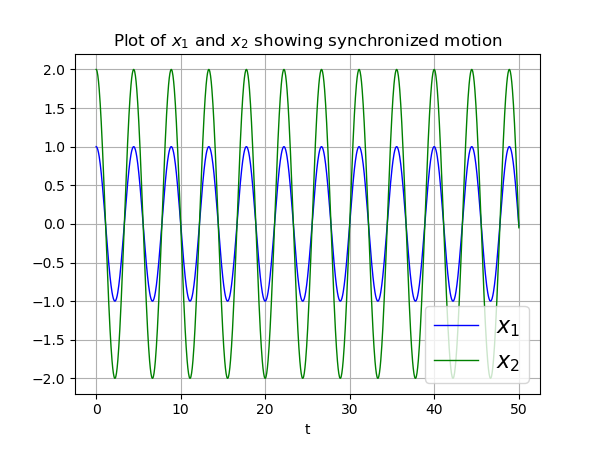
\includegraphics[width=\linewidth]{ejercicio21-sync.png}
\caption{Movimiento de $x_1$ y $x_2$ sincronizado}
\end{figure}

\begin{figure}[ht!]
	\begin{subfigure}[b]{0.5\linewidth}
    \raggedleft
	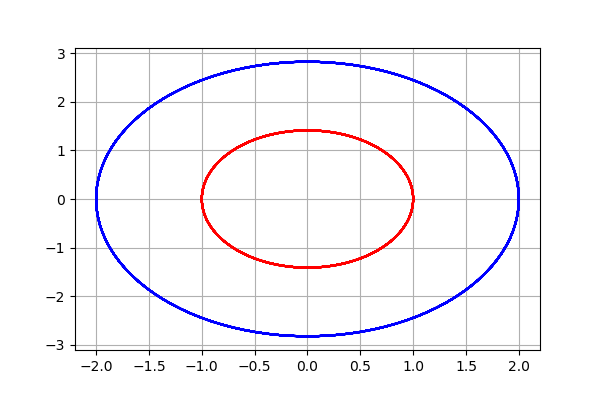
\includegraphics[width=\linewidth]{ejercicio21-phase.png}
    \caption{Retratos de fase para $x_1$ y $x_2$}
	\end{subfigure}
	\begin{subfigure}[b]{0.5\linewidth}
    \raggedright
	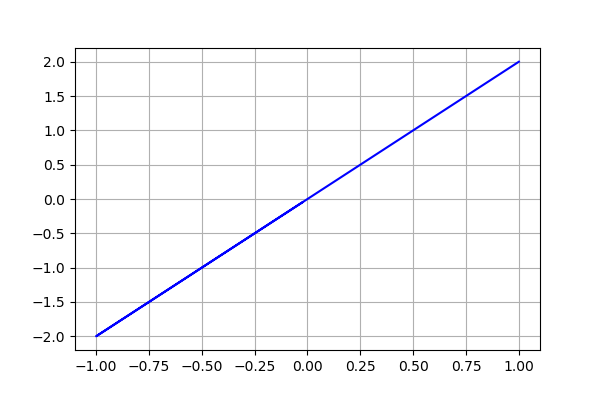
\includegraphics[width=\linewidth]{ejercicio21-versus.png}
	\caption{Relación del movimiento de $x_1$ con $x_2$}
    \end{subfigure}
\end{figure}

\newpage

\subsubsection*{\textit{Ejemplo 2.2}}

En este ejemplo se nos pide describir el movimiento de un sistema de resortes con constantes $k_1=6$ y $k_2=4$ y condiciones iniciales $(x_1,\dot{x}_1,x_2,\dot{x}_2)=(-2,0,1,0)$. De acuerdo al método analítico, la solución para el movimiento del sistema es:
\[ x_1(t)=-2\cos2\sqrt{3}t \]
\[ x_2(t)=\cos2\sqrt{3}t \]

En este ejercicio se obtuvieron los siguientes resultados para 25 segundos en 1250 particiones.

\begin{figure}[ht!]
	\begin{subfigure}[b]{0.5\linewidth}
    \raggedleft
	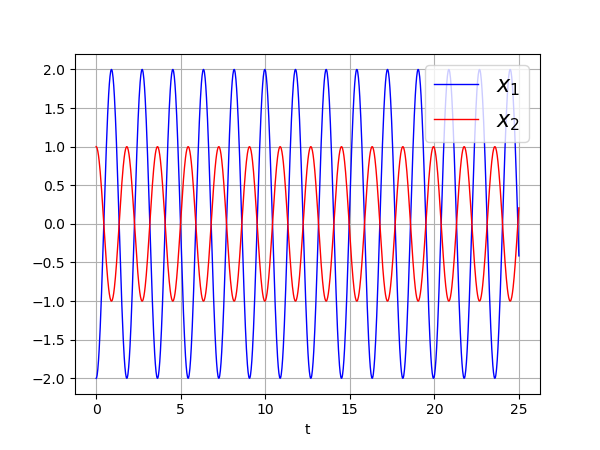
\includegraphics[width=\linewidth]{ejercicio22-sync.png}
    \caption{Movimientos descritos por $x_1$ y $x_2$}
	\end{subfigure}
	\begin{subfigure}[b]{0.5\linewidth}
    \raggedright
	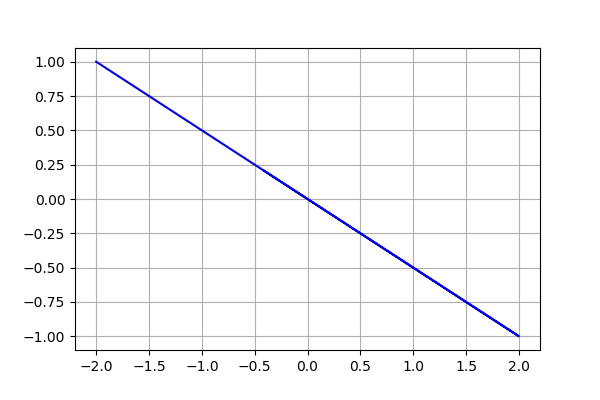
\includegraphics[width=\linewidth]{ejercicio22-versus.png}
	\caption{Relación del movimiento de $x_1$ con $x_2$}
    \end{subfigure}
\end{figure}

\subsubsection*{\textit{Ejemplo 2.3}}

En este ejemplo se nos pide describir el movimiento de un sistema de resortes con constantes $k_1=0.4$ y $k_2=1.808$ y condiciones iniciales $(x_1,\dot{x}_1,x_2,\dot{x}_2)=(1/2,0,-1/2,7/10)$. En este ejercicio se ha proporcionado a la segunda masa con una velocidad inicial

En este ejercicio se obtuvieron los siguientes resultados para 50 segundos en 1250 particiones.

\begin{figure}[h!]
	\begin{subfigure}[b]{0.5\linewidth}
    \raggedleft
	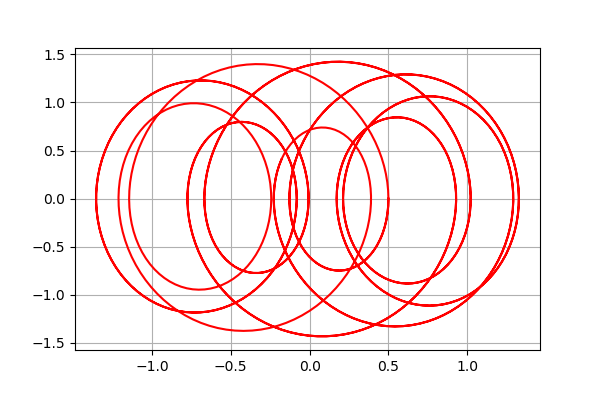
\includegraphics[width=\linewidth]{ejercicio23-phase-x1.png}
    \caption{retrato de fase de $x_1$}
	\end{subfigure}
	\begin{subfigure}[b]{0.5\linewidth}
    \raggedright
	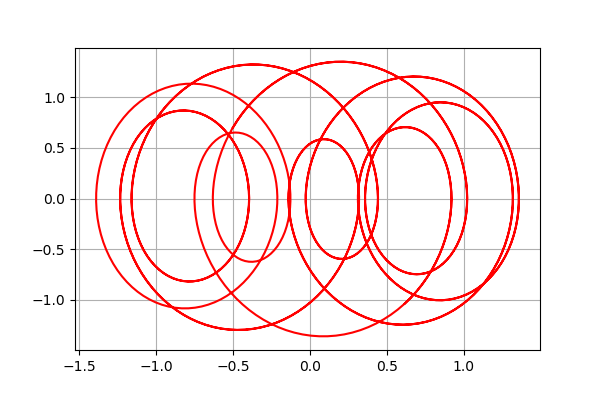
\includegraphics[width=\linewidth]{ejercicio23-phase-x2.png}
	\caption{retrato de fase de $x_2$}
    \end{subfigure}
\end{figure}

\begin{figure}[ht!]
	\begin{subfigure}[b]{0.5\linewidth}
    \raggedleft
	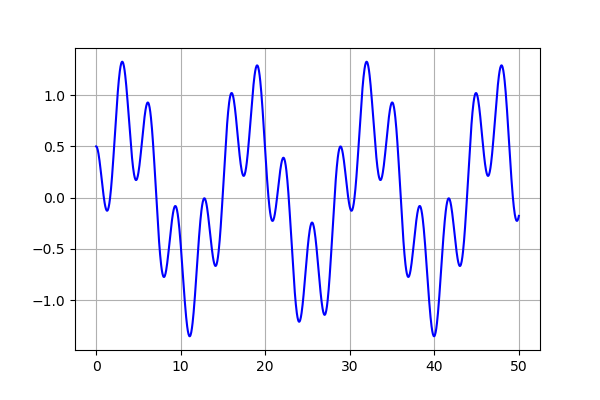
\includegraphics[width=\linewidth]{ejercicio21-x1.png}
    \caption{gráfica del movimiento de $x_1$}
	\end{subfigure}
	\begin{subfigure}[b]{0.5\linewidth}
    \raggedright
	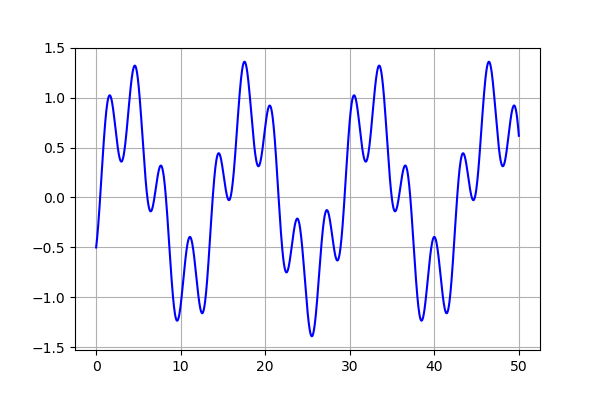
\includegraphics[width=\linewidth]{ejercicio21-x2.png}
	\caption{gráfica del movimiento de $x_2$}
    \end{subfigure}
\end{figure}

\begin{figure}[ht!]
	\begin{subfigure}[b]{0.5\linewidth}
    \raggedleft
	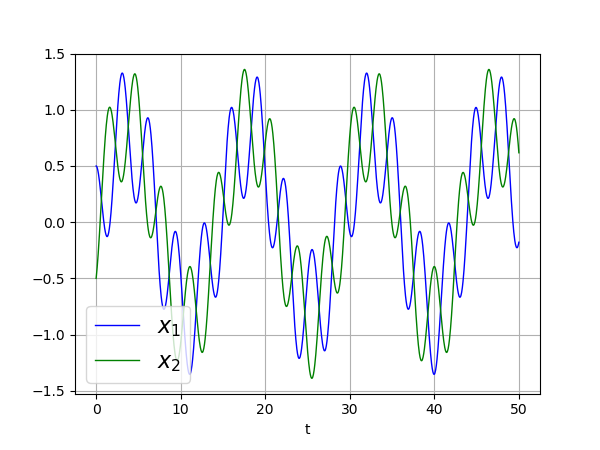
\includegraphics[width=\linewidth]{ejercicio23-sync.png}
    \caption{movimiento de ambas masas, $x_1$ y $x_2$}
	\end{subfigure}
	\begin{subfigure}[b]{0.5\linewidth}
    \raggedright
	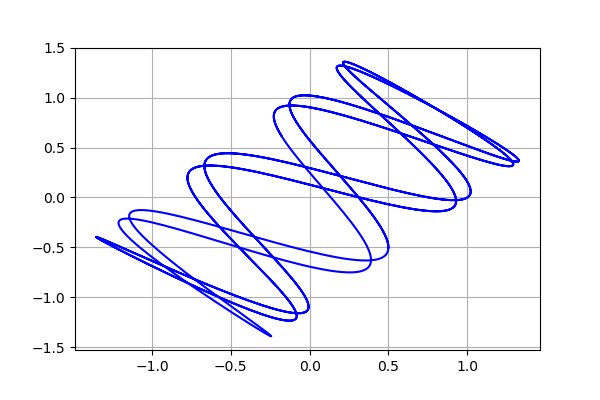
\includegraphics[width=\linewidth]{ejercicio23-versus.png}
	\caption{Relación del movimiento de $x_1$ con $x_2$}
    \end{subfigure}
\end{figure}

\newpage

\subsubsection{Amortiguamiento}

\subsubsection*{\textit{Ejemplo 2.4}}

En este ejemplo se nos pide describir el movimiento de un sistema de resortes con constantes $k_1=0.4$ y $k_2=1.808$, con coeficientes de fricción $b_1=0.1$ y $b_2=0.2$ y condiciones iniciales $(x_1,\dot{x}_1,x_2,\dot{x}_2)=(1,1/2,2,1/2)$. En este ejercicio se han introducido los efectos de amortiguamiento al cambiar los parametros $b_1$ y $b_2$.

En este ejercicio se obtuvieron los siguientes resultados para 50 segundos en 1250 particiones.

\begin{figure}[ht!]
	\begin{subfigure}[b]{0.5\linewidth}
    \raggedleft
	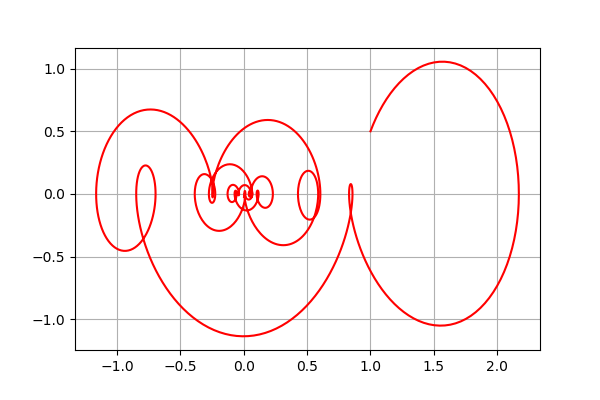
\includegraphics[width=\linewidth]{ejercicio24-phase-x1.png}
    \caption{retrato de fase de $x_1$}
	\end{subfigure}
	\begin{subfigure}[b]{0.5\linewidth}
    \raggedright
	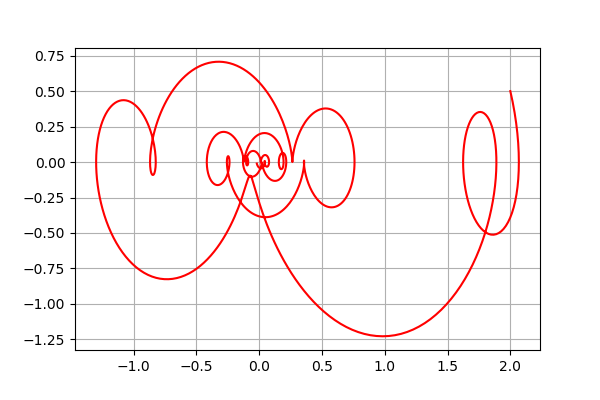
\includegraphics[width=\linewidth]{ejercicio24-phase-x2.png}
	\caption{retrato de fase de $x_2$}
    \end{subfigure}
\end{figure}

\begin{figure}[ht!]
	\begin{subfigure}[b]{0.5\linewidth}
    \raggedleft
	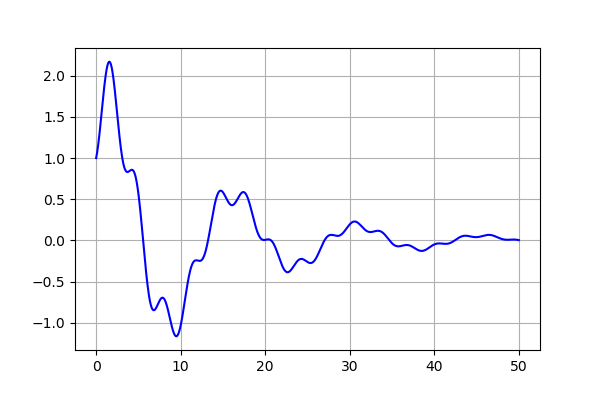
\includegraphics[width=\linewidth]{ejercicio24-x1.png}
    \caption{gráfica del movimiento de $x_1$}
	\end{subfigure}
	\begin{subfigure}[b]{0.5\linewidth}
    \raggedright
	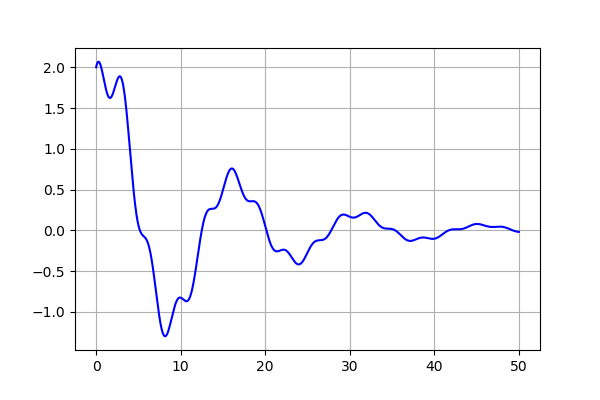
\includegraphics[width=\linewidth]{ejercicio24-x2.png}
	\caption{gráfica del movimiento de $x_2$}
    \end{subfigure}
\end{figure}

\begin{figure}[ht!]
	\begin{subfigure}[b]{0.5\linewidth}
    \raggedleft
	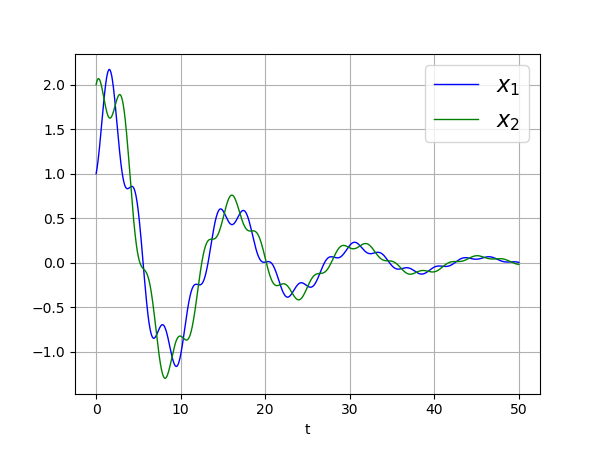
\includegraphics[width=\linewidth]{ejercicio24-sync.png}
    \caption{movimiento de ambas masas, $x_1$ y $x_2$}
	\end{subfigure}
	\begin{subfigure}[b]{0.5\linewidth}
    \raggedright
	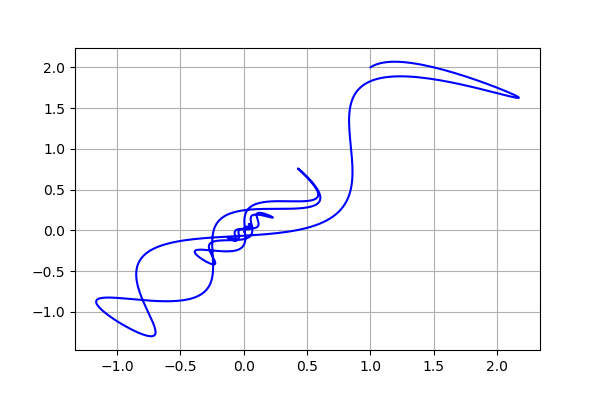
\includegraphics[width=\linewidth]{ejercicio24-versus.png}
	\caption{Relación del movimiento de $x_1$ con $x_2$}
    \end{subfigure}
\end{figure}

\newpage

\section{Resultados}

Para conocer que tan buena es nuestra aproximación de la solución requerimos calcular el error relativo de las soluciones comparandolas con las soluciones analíticas proporcionadas por el artículo de Fay \& Graham para los ejercicios 2.1 y 2.2

Para obtener el error relativo de las soluciones $x_1$ y $x_2$ en el ejercicio 2.1 añadimos la siguiente expresión a la lista de datos:
\[ e_1=\left|\frac{\cos\sqrt{2}t-x_1}{\cos\sqrt{2}t}\right| \]
\[ e_2=\left|\frac{2\cos\sqrt{2}t-x_2}{2\cos\sqrt{2}t}\right| \]

El cámbio en el código yace al imprimir la solución en un archivo:

\begin{framed}
\begin{verbatim}
with open('ejercicio21.dat', 'w') as f:
    # Print & save the solution.
    for t1, w1 in zip(t, wsol):
        print(t1, w1[0], w1[1], w1[2], w1[3],
        np.abs((w1[0]-(np.cos(np.sqrt(2)*t1)))
        /(np.cos(np.sqrt(2)*t1))),
        np.abs((w1[2]-(2*np.cos(np.sqrt(2)*t1)))
        /(2*np.cos(np.sqrt(2)*t1))),
        file=f)
\end{verbatim}
\end{framed} 

donde $x_1$ y $x_2$ son las soluciones en los momentos $t$. Esto nos dan las siguientes gráficas para los errores con respecto al tiempo:

\begin{figure}[h!]
	\begin{subfigure}[b]{0.5\linewidth}
    \raggedleft
	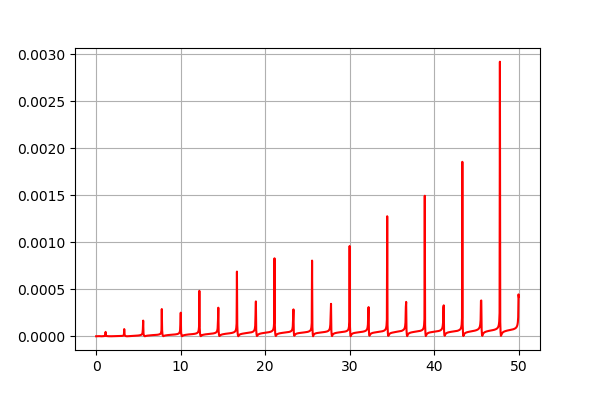
\includegraphics[width=\linewidth]{ejercicio21-error1.png}
    \caption{error relativo de la solución $x_1$}
	\end{subfigure}
	\begin{subfigure}[b]{0.5\linewidth}
    \raggedright
	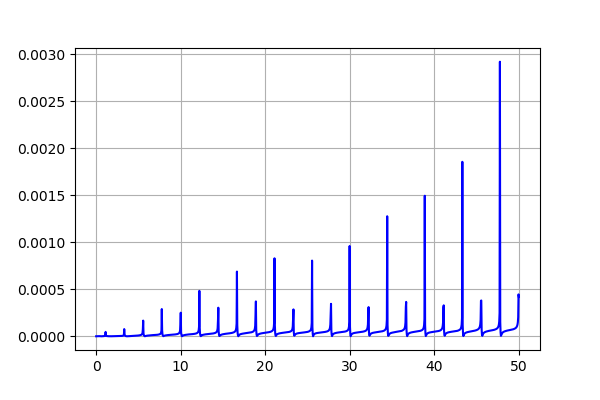
\includegraphics[width=\linewidth]{ejercicio21-error2.png}
	\caption{error relativo de la solución $x_2$}
    \end{subfigure}
    \caption{Errores para el ejercicio 2.1}
\end{figure}

Se realizó el mismo proceso para el ejercicio 2.2 con las expresiones para el error relativo correspondientes:

\[ e_1=\left|\frac{2\cos2\sqrt{3}t-x_1}{2\cos2\sqrt{3}t}\right| \]
\[ e_2=\left|\frac{\cos2\sqrt{3}t-x_2}{\cos2\sqrt{3}t}\right| \]

Obtuvimos las siguientes gráficas para los errores de las soluciones:

\begin{figure}[h!]
	\begin{subfigure}[b]{0.5\linewidth}
    \raggedleft
	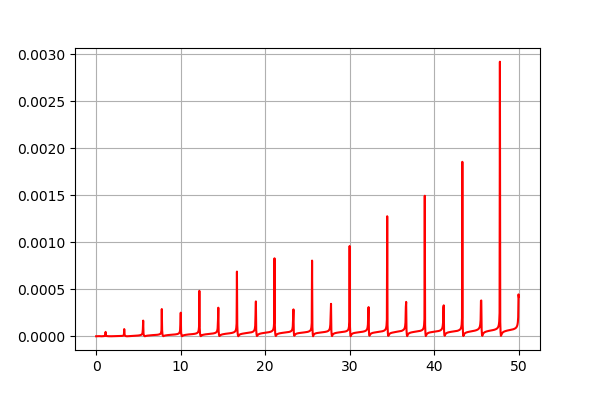
\includegraphics[width=\linewidth]{ejercicio21-error1.png}
    \caption{error relativo de la solución $x_1$}
	\end{subfigure}
	\begin{subfigure}[b]{0.5\linewidth}
    \raggedright
	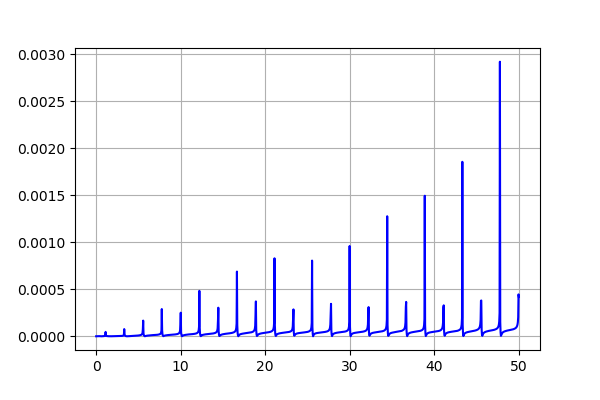
\includegraphics[width=\linewidth]{ejercicio21-error2.png}
	\caption{error relativo de la solución $x_2$}
    \end{subfigure}
    \caption{Errores para el ejercicio 2.2}
\end{figure}

\section{Conclusión}

Con esto podemos darnos cuenta que Python es una buena herramienta para buscar soluciones numéricas de sistemas de ecuaciones diferenciales ordinarias para gráficar

Se pueden obtener gráficas que se aprecian correctamente aparte de que se pueden manejar fácilmente.
\newpage

\section{Bibliografía}
\begin{itemize}
\item The Scipy community. (Oct 25, 2017). Integration and ODE's (scipy.integrate). Mar 18, 2018, de The Scipy community Sitio web: https://docs.scipy.org/doc/scipy/reference/integrate.html

\item TEMPLE H. FAY, SARAH DUNCAN GRAHAM. (12 September 2002). Coupled spring equations. En int. j. math. educ. sci. technol., 2003(65–79). attiesburg, MS: Taylor \& Francis. 
\end{itemize}

\newpage

\title{\textbf{Apéndice}}

\begin{enumerate}
\item ¿En general te pareció interesante esta actividad de modelación matemática? ¿Qué te gustó mas? ¿Qué no te gustó? ~\\~\\
En general me parece interesante que Python pueda resolver sistemas de ecuaciones diferenciales utilizando ODEint.
Me gustó el hecho de que pudimos obtener distintas soluciones particulares y gráficarlas con tan solo cambiar los valores parámetros o condiciones iniciales en una sección donde se encontraban contenidas.
Lo que menos me gustó es que no tuvimos un tipo de introducción al código necesario para resolver los sistemas, solo le entramos y ya

\item La cantidad de material te pareció ¿bien?, ¿suficiente?, ¿demasiado?~\\~\\
Me pareció suficiente

\item ¿Cuál es tu primera impresión de Jupyter Lab? ~\\~\\
Esta bastante facil de manejar y es conveniente tener el menú con las pestañas al mismo tiempo que editamos con todos los comandos en la barra de al lado

\item Respecto al uso de funciones de SciPy, ¿ya habías visto integración numérica en tus cursos anteriores? ¿Cuál es tu experiencia?  ~\\~\\
Si pero no para resolver ecuaciones diferenciales ordinarias

\item El tema de sistema de masas acopladas con resortes, ¿ya lo habías resuelto en tu curso de Mecánica 2?  ~\\~\\
Así es, sólo que únicamente lo resolvimos sin amortiguamiento o forzamiento

\item ¿Qué le quitarías o agregarías a esta actividad para hacerla más interesante y divertida? ~\\~\\
no lo se 


\end{enumerate}

\end{document}
